\documentclass[twoside]{book}

% Packages required by doxygen
\usepackage{calc}
\usepackage{doxygen}
\usepackage{graphicx}
\usepackage[utf8]{inputenc}
\usepackage{makeidx}
\usepackage{multicol}
\usepackage{multirow}
\usepackage{textcomp}
\usepackage[table]{xcolor}

% Font selection
\usepackage[T1]{fontenc}
\usepackage{mathptmx}
\usepackage[scaled=.90]{helvet}
\usepackage{courier}
\usepackage{amssymb}
\usepackage{sectsty}
\renewcommand{\familydefault}{\sfdefault}
\allsectionsfont{%
  \fontseries{bc}\selectfont%
  \color{darkgray}%
}
\renewcommand{\DoxyLabelFont}{%
  \fontseries{bc}\selectfont%
  \color{darkgray}%
}

% Page & text layout
\usepackage{geometry}
\geometry{%
  a4paper,%
  top=2.5cm,%
  bottom=2.5cm,%
  left=2.5cm,%
  right=2.5cm%
}
\tolerance=750
\hfuzz=15pt
\hbadness=750
\setlength{\emergencystretch}{15pt}
\setlength{\parindent}{0cm}
\setlength{\parskip}{0.2cm}
\makeatletter
\renewcommand{\paragraph}{%
  \@startsection{paragraph}{4}{0ex}{-1.0ex}{1.0ex}{%
    \normalfont\normalsize\bfseries\SS@parafont%
  }%
}
\renewcommand{\subparagraph}{%
  \@startsection{subparagraph}{5}{0ex}{-1.0ex}{1.0ex}{%
    \normalfont\normalsize\bfseries\SS@subparafont%
  }%
}
\makeatother

% Headers & footers
\usepackage{fancyhdr}
\pagestyle{fancyplain}
\fancyhead[LE]{\fancyplain{}{\bfseries\thepage}}
\fancyhead[CE]{\fancyplain{}{}}
\fancyhead[RE]{\fancyplain{}{\bfseries\leftmark}}
\fancyhead[LO]{\fancyplain{}{\bfseries\rightmark}}
\fancyhead[CO]{\fancyplain{}{}}
\fancyhead[RO]{\fancyplain{}{\bfseries\thepage}}
\fancyfoot[LE]{\fancyplain{}{}}
\fancyfoot[CE]{\fancyplain{}{}}
\fancyfoot[RE]{\fancyplain{}{\bfseries\scriptsize Generated on Tue Dec 3 2013 23\-:41\-:13 for Trial1 by Doxygen }}
\fancyfoot[LO]{\fancyplain{}{\bfseries\scriptsize Generated on Tue Dec 3 2013 23\-:41\-:13 for Trial1 by Doxygen }}
\fancyfoot[CO]{\fancyplain{}{}}
\fancyfoot[RO]{\fancyplain{}{}}
\renewcommand{\footrulewidth}{0.4pt}
\renewcommand{\chaptermark}[1]{%
  \markboth{#1}{}%
}
\renewcommand{\sectionmark}[1]{%
  \markright{\thesection\ #1}%
}

% Indices & bibliography
\usepackage{natbib}
\usepackage[titles]{tocloft}
\setcounter{tocdepth}{3}
\setcounter{secnumdepth}{5}
\makeindex

% Hyperlinks (required, but should be loaded last)
\usepackage{ifpdf}
\ifpdf
  \usepackage[pdftex,pagebackref=true]{hyperref}
\else
  \usepackage[ps2pdf,pagebackref=true]{hyperref}
\fi
\hypersetup{%
  colorlinks=true,%
  linkcolor=blue,%
  citecolor=blue,%
  unicode%
}

% Custom commands
\newcommand{\clearemptydoublepage}{%
  \newpage{\pagestyle{empty}\cleardoublepage}%
}


%===== C O N T E N T S =====

\begin{document}

% Titlepage & ToC
\hypersetup{pageanchor=false}
\pagenumbering{roman}
\begin{titlepage}
\vspace*{7cm}
\begin{center}%
{\Large Trial1 }\\
\vspace*{1cm}
{\large Generated by Doxygen 1.8.5}\\
\vspace*{0.5cm}
{\small Tue Dec 3 2013 23:41:13}\\
\end{center}
\end{titlepage}
\clearemptydoublepage
\tableofcontents
\clearemptydoublepage
\pagenumbering{arabic}
\hypersetup{pageanchor=true}

%--- Begin generated contents ---
\chapter{M\-J\-Baking\-Quest}
\label{md__c_1__users__joslyn__documents__git_hub__m_j_baking_quest__r_e_a_d_m_e}
\hypertarget{md__c_1__users__joslyn__documents__git_hub__m_j_baking_quest__r_e_a_d_m_e}{}
This is the repository for our C\-S340 semester project. 
\chapter{Hierarchical Index}
\section{Class Hierarchy}
This inheritance list is sorted roughly, but not completely, alphabetically\-:\begin{DoxyCompactList}
\item \contentsline{section}{engine}{\pageref{classengine}}{}
\item \contentsline{section}{Node}{\pageref{class_node}}{}
\item \contentsline{section}{obj\-Structure}{\pageref{classobj_structure}}{}
\item \contentsline{section}{parser}{\pageref{classparser}}{}
\item Q\-Graphics\-View\begin{DoxyCompactList}
\item \contentsline{section}{Graphics\-View}{\pageref{class_graphics_view}}{}
\begin{DoxyCompactList}
\item \contentsline{section}{Graphics\-View\-Editor}{\pageref{class_graphics_view_editor}}{}
\end{DoxyCompactList}
\end{DoxyCompactList}
\item Q\-Graphics\-Widget\begin{DoxyCompactList}
\item \contentsline{section}{Q\-Graphics\-Rect\-Widget}{\pageref{class_q_graphics_rect_widget}}{}
\end{DoxyCompactList}
\item Q\-Main\-Window\begin{DoxyCompactList}
\item \contentsline{section}{edit\-Window}{\pageref{classedit_window}}{}
\item \contentsline{section}{gamewindow}{\pageref{classgamewindow}}{}
\item \contentsline{section}{Main\-Window}{\pageref{class_main_window}}{}
\end{DoxyCompactList}
\item Q\-Message\-Box\begin{DoxyCompactList}
\item \contentsline{section}{My\-Message\-Box}{\pageref{class_my_message_box}}{}
\end{DoxyCompactList}
\item Q\-Widget\begin{DoxyCompactList}
\item \contentsline{section}{start}{\pageref{classstart}}{}
\end{DoxyCompactList}
\end{DoxyCompactList}

\chapter{Class Index}
\section{Class List}
Here are the classes, structs, unions and interfaces with brief descriptions\-:\begin{DoxyCompactList}
\item\contentsline{section}{\hyperlink{classedit_window}{edit\-Window} }{\pageref{classedit_window}}{}
\item\contentsline{section}{\hyperlink{classengine}{engine} }{\pageref{classengine}}{}
\item\contentsline{section}{\hyperlink{classgamewindow}{gamewindow} }{\pageref{classgamewindow}}{}
\item\contentsline{section}{\hyperlink{class_graphics_view}{Graphics\-View} }{\pageref{class_graphics_view}}{}
\item\contentsline{section}{\hyperlink{class_graphics_view_editor}{Graphics\-View\-Editor} }{\pageref{class_graphics_view_editor}}{}
\item\contentsline{section}{\hyperlink{class_main_window}{Main\-Window} }{\pageref{class_main_window}}{}
\item\contentsline{section}{\hyperlink{class_my_message_box}{My\-Message\-Box} }{\pageref{class_my_message_box}}{}
\item\contentsline{section}{\hyperlink{class_node}{Node} }{\pageref{class_node}}{}
\item\contentsline{section}{\hyperlink{classobj_structure}{obj\-Structure} }{\pageref{classobj_structure}}{}
\item\contentsline{section}{\hyperlink{classparser}{parser} }{\pageref{classparser}}{}
\item\contentsline{section}{\hyperlink{class_q_graphics_rect_widget}{Q\-Graphics\-Rect\-Widget} }{\pageref{class_q_graphics_rect_widget}}{}
\item\contentsline{section}{\hyperlink{classstart}{start} }{\pageref{classstart}}{}
\end{DoxyCompactList}

\chapter{Class Documentation}
\hypertarget{classedit_window}{\section{edit\-Window Class Reference}
\label{classedit_window}\index{edit\-Window@{edit\-Window}}
}
Inheritance diagram for edit\-Window\-:\begin{figure}[H]
\begin{center}
\leavevmode
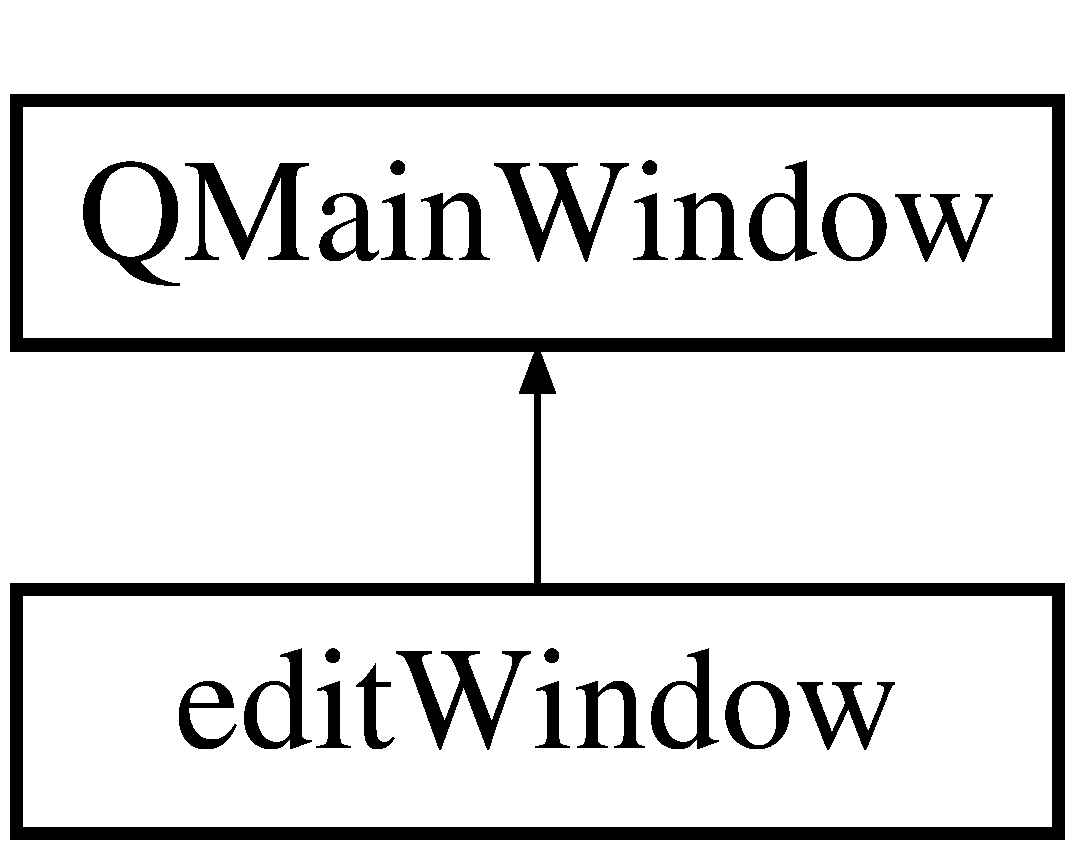
\includegraphics[height=2.000000cm]{classedit_window}
\end{center}
\end{figure}
\subsection*{Public Member Functions}
\begin{DoxyCompactItemize}
\item 
\hypertarget{classedit_window_a3584b9b685c463d050ce2925c13a44e7}{Q\-Graphics\-View $\ast$ {\bfseries Get\-Graphics\-View} ()}\label{classedit_window_a3584b9b685c463d050ce2925c13a44e7}

\item 
\hypertarget{classedit_window_aefaed4216416797acd5ade0da432f4dc}{Q\-Graphics\-Scene $\ast$ {\bfseries Get\-Graphics\-Scene} ()}\label{classedit_window_aefaed4216416797acd5ade0da432f4dc}

\item 
\hyperlink{classedit_window_a494969043b61ec9664804df9253cb8c9}{edit\-Window} (Q\-Widget $\ast$parent=0)
\begin{DoxyCompactList}\small\item\em editwindow\-::edit\-Window Uses \hyperlink{class_graphics_view}{Graphics\-View} to display level editor window. Calls engine to generate items for window. \end{DoxyCompactList}\item 
\hypertarget{classedit_window_a39528533eb2ffcc4a8442b3c02eb1ffd}{void {\bfseries Init\-Graphics} (Q\-Graphics\-Scene $\ast$scene)}\label{classedit_window_a39528533eb2ffcc4a8442b3c02eb1ffd}

\item 
\hypertarget{classedit_window_a0fc9d66a5d73435b5d1bf5626a8862c9}{\hyperlink{classedit_window_a0fc9d66a5d73435b5d1bf5626a8862c9}{$\sim$edit\-Window} ()}\label{classedit_window_a0fc9d66a5d73435b5d1bf5626a8862c9}

\begin{DoxyCompactList}\small\item\em \hyperlink{classedit_window_a0fc9d66a5d73435b5d1bf5626a8862c9}{edit\-Window\-::$\sim$edit\-Window} To clean up stuff when your done! \end{DoxyCompactList}\end{DoxyCompactItemize}


\subsection{Constructor \& Destructor Documentation}
\hypertarget{classedit_window_a494969043b61ec9664804df9253cb8c9}{\index{edit\-Window@{edit\-Window}!edit\-Window@{edit\-Window}}
\index{edit\-Window@{edit\-Window}!editWindow@{edit\-Window}}
\subsubsection[{edit\-Window}]{\setlength{\rightskip}{0pt plus 5cm}edit\-Window\-::edit\-Window (
\begin{DoxyParamCaption}
\item[{Q\-Widget $\ast$}]{parent = {\ttfamily 0}}
\end{DoxyParamCaption}
)\hspace{0.3cm}{\ttfamily [explicit]}}}\label{classedit_window_a494969043b61ec9664804df9253cb8c9}


editwindow\-::edit\-Window Uses \hyperlink{class_graphics_view}{Graphics\-View} to display level editor window. Calls engine to generate items for window. 

editwindow\-::edit\-Window This class sets up the window of the level editor. This window includes menus for help, tools to build a level and a file menu. 

The documentation for this class was generated from the following files\-:\begin{DoxyCompactItemize}
\item 
Doxygen/editormainwindow.\-h\item 
Doxygen/editormainwindow.\-cpp\end{DoxyCompactItemize}

\hypertarget{classengine}{\section{engine Class Reference}
\label{classengine}\index{engine@{engine}}
}
\subsection*{Public Member Functions}
\begin{DoxyCompactItemize}
\item 
\hypertarget{classengine_aaffbfa4e20b4b627f2336eb6b40db348}{\hyperlink{classengine_aaffbfa4e20b4b627f2336eb6b40db348}{engine} ()}\label{classengine_aaffbfa4e20b4b627f2336eb6b40db348}

\begin{DoxyCompactList}\small\item\em \hyperlink{classengine_aaffbfa4e20b4b627f2336eb6b40db348}{engine\-::engine} Creates all objects defined in the parser for each level. It also keeps track of how many walkable objects (M\-J, good guys, enemies) and hearts (for the health bar) are to appear in the level. \end{DoxyCompactList}\item 
\hypertarget{classengine_a5fc1dc660b130df073d776e17f443ef5}{{\bfseries engine} (Q\-Graphics\-Scene $\ast$scene)}\label{classengine_a5fc1dc660b130df073d776e17f443ef5}

\item 
\hypertarget{classengine_aeaac5db377f37a85bfae53711e8248c0}{Q\-Graphics\-Scene $\ast$ \hyperlink{classengine_aeaac5db377f37a85bfae53711e8248c0}{Get\-Scene} ()}\label{classengine_aeaac5db377f37a85bfae53711e8248c0}

\begin{DoxyCompactList}\small\item\em \hyperlink{classengine_aeaac5db377f37a85bfae53711e8248c0}{engine\-::\-Get\-Scene} returns a pointer to the current graphics scene \end{DoxyCompactList}\item 
\hypertarget{classengine_a0421c21bd062075ab965333e05f20626}{void {\bfseries Set\-Scene} (Q\-Graphics\-Scene $\ast$scene)}\label{classengine_a0421c21bd062075ab965333e05f20626}

\item 
\hypertarget{classengine_ad0d2625e9b6f5b9ed18df6076001ea73}{void {\bfseries Set\-Parent\-Window} (Q\-Widget $\ast$p\-Window)}\label{classengine_ad0d2625e9b6f5b9ed18df6076001ea73}

\item 
\hypertarget{classengine_a4e8515e2f893531685ab028f42567137}{void \hyperlink{classengine_a4e8515e2f893531685ab028f42567137}{load\-Game} (Q\-String level)}\label{classengine_a4e8515e2f893531685ab028f42567137}

\begin{DoxyCompactList}\small\item\em \hyperlink{classengine_a4e8515e2f893531685ab028f42567137}{engine\-::load\-Game} loads level without the file chooser, for now default level \end{DoxyCompactList}\item 
\hypertarget{classengine_a6e3fca96515e269117b4cc46750f363e}{void \hyperlink{classengine_a6e3fca96515e269117b4cc46750f363e}{save\-Game} (Q\-String name)}\label{classengine_a6e3fca96515e269117b4cc46750f363e}

\begin{DoxyCompactList}\small\item\em \hyperlink{classengine_a6e3fca96515e269117b4cc46750f363e}{engine\-::save\-Game} Created a file with the current map and status of the game. This method does the reverse of Load\-Map where instead od loading the objects from the map file, it creates a map file with the object in the level and the the states they are in. \end{DoxyCompactList}\item 
\hypertarget{classengine_a02ad5e7f4d1073a97f77d153c9685ff8}{void \hyperlink{classengine_a02ad5e7f4d1073a97f77d153c9685ff8}{Clicked\-Open\-Map} (void)}\label{classengine_a02ad5e7f4d1073a97f77d153c9685ff8}

\begin{DoxyCompactList}\small\item\em \hyperlink{classengine_a02ad5e7f4d1073a97f77d153c9685ff8}{engine\-::\-Clicked\-Open\-Map} Opens the file chooser dialog and loads the map \end{DoxyCompactList}\item 
\hypertarget{classengine_ae322ec44826013a47ac954f9b8fc24b2}{void \hyperlink{classengine_ae322ec44826013a47ac954f9b8fc24b2}{Clicked\-Save\-Map} (void)}\label{classengine_ae322ec44826013a47ac954f9b8fc24b2}

\begin{DoxyCompactList}\small\item\em \hyperlink{classengine_ae322ec44826013a47ac954f9b8fc24b2}{engine\-::\-Clicked\-Save\-Map} Opens the file save dialog and allows user to save current level to a new file, or overwrite an already saved file \end{DoxyCompactList}\item 
\hypertarget{classengine_a68b46ec574d97c62f29206fd201b34b5}{void \hyperlink{classengine_a68b46ec574d97c62f29206fd201b34b5}{Close\-Map} (void)}\label{classengine_a68b46ec574d97c62f29206fd201b34b5}

\begin{DoxyCompactList}\small\item\em \hyperlink{classengine_a68b46ec574d97c62f29206fd201b34b5}{engine\-::\-Close\-Map} Clears out the scene \end{DoxyCompactList}\item 
\hypertarget{classengine_aff95606d7fa78ddd3f13b0573d8fa284}{void {\bfseries Clicked\-Draw\-Grid\-Lines} (void)}\label{classengine_aff95606d7fa78ddd3f13b0573d8fa284}

\item 
\hypertarget{classengine_a804d510d34deaebcfff0bf5af93568ec}{void \hyperlink{classengine_a804d510d34deaebcfff0bf5af93568ec}{Add\-Sprite} (const char $\ast$sprite\-F\-Name, int x\-Loc, int y\-Loc)}\label{classengine_a804d510d34deaebcfff0bf5af93568ec}

\begin{DoxyCompactList}\small\item\em \hyperlink{classengine_a804d510d34deaebcfff0bf5af93568ec}{engine\-::\-Add\-Sprite} Creates a widget for sprites, givien a sprite picture, and a position. The sprite also holds properties that tell wheter or not it is a movable object. \end{DoxyCompactList}\item 
\hypertarget{classengine_ac084e69968320aa57383fc251f54b887}{void \hyperlink{classengine_ac084e69968320aa57383fc251f54b887}{move\-Char} (int direction)}\label{classengine_ac084e69968320aa57383fc251f54b887}

\begin{DoxyCompactList}\small\item\em \hyperlink{classengine_ac084e69968320aa57383fc251f54b887}{engine\-::move\-Char} method that is used to move mj. This method changes her sprite picture and updates her posistion \end{DoxyCompactList}\item 
\hypertarget{classengine_ab27f5792c30dfd6e6cc4fcfd390d15eb}{void \hyperlink{classengine_ab27f5792c30dfd6e6cc4fcfd390d15eb}{move\-Enemies} ()}\label{classengine_ab27f5792c30dfd6e6cc4fcfd390d15eb}

\begin{DoxyCompactList}\small\item\em \hyperlink{classengine_ab27f5792c30dfd6e6cc4fcfd390d15eb}{engine\-::move\-Enemies} moves the good characters \end{DoxyCompactList}\item 
\hypertarget{classengine_ad010e22061b9a72eb0ff69821ffbfbc6}{void \hyperlink{classengine_ad010e22061b9a72eb0ff69821ffbfbc6}{move\-Good} ()}\label{classengine_ad010e22061b9a72eb0ff69821ffbfbc6}

\begin{DoxyCompactList}\small\item\em \hyperlink{classengine_ad010e22061b9a72eb0ff69821ffbfbc6}{engine\-::move\-Good} moves the good characters \end{DoxyCompactList}\item 
\hypertarget{classengine_a3fc3e6605e74eb8ba71316b15471a1c3}{void \hyperlink{classengine_a3fc3e6605e74eb8ba71316b15471a1c3}{get\-Block} ()}\label{classengine_a3fc3e6605e74eb8ba71316b15471a1c3}

\begin{DoxyCompactList}\small\item\em \hyperlink{classengine_a3fc3e6605e74eb8ba71316b15471a1c3}{engine\-::get\-Block} allows M\-J to pick up blocks below her (when she is facing front) or on the right or left of her, depending on which direction she is facing \end{DoxyCompactList}\item 
\hypertarget{classengine_ac37f50e0ee7aa83b113d8e4dbd9ee069}{void \hyperlink{classengine_ac37f50e0ee7aa83b113d8e4dbd9ee069}{drop\-Block} ()}\label{classengine_ac37f50e0ee7aa83b113d8e4dbd9ee069}

\begin{DoxyCompactList}\small\item\em \hyperlink{classengine_ac37f50e0ee7aa83b113d8e4dbd9ee069}{engine\-::drop\-Block()} using mj's position we find the position of the block she is carrying and check to see if the place where the player wants to drop it is a legal place, ie there is no block there. If block lands on an enemy, they die (disappear) \end{DoxyCompactList}\item 
\hypertarget{classengine_a56c6f2331fa2045f184b183c89f9c199}{void \hyperlink{classengine_a56c6f2331fa2045f184b183c89f9c199}{load\-Next} ()}\label{classengine_a56c6f2331fa2045f184b183c89f9c199}

\begin{DoxyCompactList}\small\item\em \hyperlink{classengine_a56c6f2331fa2045f184b183c89f9c199}{engine\-::load\-Next} checks if mj is by the door if she is then load the next level \end{DoxyCompactList}\item 
\hypertarget{classengine_a1fa4f5009e031570cd0e40d7056c8a61}{void \hyperlink{classengine_a1fa4f5009e031570cd0e40d7056c8a61}{check\-Collisions} ()}\label{classengine_a1fa4f5009e031570cd0e40d7056c8a61}

\begin{DoxyCompactList}\small\item\em engine\-::check\-Collision() checks to see if M\-J collides with any of the people if she collides with a good guy, she gets the item they are holding if she collides with an enemy, she loses a life, until she runs out when she runs out the game resets to the beginning of that level \end{DoxyCompactList}\item 
\hypertarget{classengine_a6ffdddfa828e97da265f0483509f7554}{void \hyperlink{classengine_a6ffdddfa828e97da265f0483509f7554}{start\-Over} ()}\label{classengine_a6ffdddfa828e97da265f0483509f7554}

\begin{DoxyCompactList}\small\item\em \hyperlink{classengine_ac084e69968320aa57383fc251f54b887}{engine\-::move\-Char} starts the current level over by first clearing out the life and then callong reset \end{DoxyCompactList}\end{DoxyCompactItemize}
\subsection*{Public Attributes}
\begin{DoxyCompactItemize}
\item 
\hypertarget{classengine_ab3a51856b749c44d32f45ab4ba653d59}{\hyperlink{class_node}{Node} $\ast$ {\bfseries mj}}\label{classengine_ab3a51856b749c44d32f45ab4ba653d59}

\item 
\hypertarget{classengine_ab994ab325c0c9fa80dea14e935f20d83}{\hyperlink{class_node}{Node} $\ast$ {\bfseries walkable} \mbox{[}20\mbox{]}\mbox{[}30\mbox{]}}\label{classengine_ab994ab325c0c9fa80dea14e935f20d83}

\item 
\hypertarget{classengine_a3f98c76f5a03777bd0e0543dae1c9725}{\hyperlink{class_q_graphics_rect_widget}{Q\-Graphics\-Rect\-Widget} $\ast$ {\bfseries good\-Obj} \mbox{[}5\mbox{]}}\label{classengine_a3f98c76f5a03777bd0e0543dae1c9725}

\item 
\hypertarget{classengine_a66bf076777496c5588df19a7191bbdb4}{bool {\bfseries mj\-Has\-Block}}\label{classengine_a66bf076777496c5588df19a7191bbdb4}

\item 
\hypertarget{classengine_a4a40819a98ac7ab07ce6669a291adfaf}{int {\bfseries item\-Count}}\label{classengine_a4a40819a98ac7ab07ce6669a291adfaf}

\item 
\hypertarget{classengine_a03e0b46f80c31f67235837a8cbb9ee27}{int {\bfseries life}}\label{classengine_a03e0b46f80c31f67235837a8cbb9ee27}

\item 
\hypertarget{classengine_ab72a971b9c7b2c4206a8d27c5a26f83d}{\hyperlink{classobj_structure}{obj\-Structure} $\ast$ {\bfseries blocks}}\label{classengine_ab72a971b9c7b2c4206a8d27c5a26f83d}

\item 
\hypertarget{classengine_a5d5f9c8f20bc2e91e4bba4afac71dbad}{\hyperlink{classparser}{parser} $\ast$ {\bfseries parsley}}\label{classengine_a5d5f9c8f20bc2e91e4bba4afac71dbad}

\end{DoxyCompactItemize}


The documentation for this class was generated from the following files\-:\begin{DoxyCompactItemize}
\item 
engine.\-h\item 
engine.\-cpp\end{DoxyCompactItemize}

\hypertarget{classgamewindow}{\section{gamewindow Class Reference}
\label{classgamewindow}\index{gamewindow@{gamewindow}}
}
Inheritance diagram for gamewindow\-:\begin{figure}[H]
\begin{center}
\leavevmode
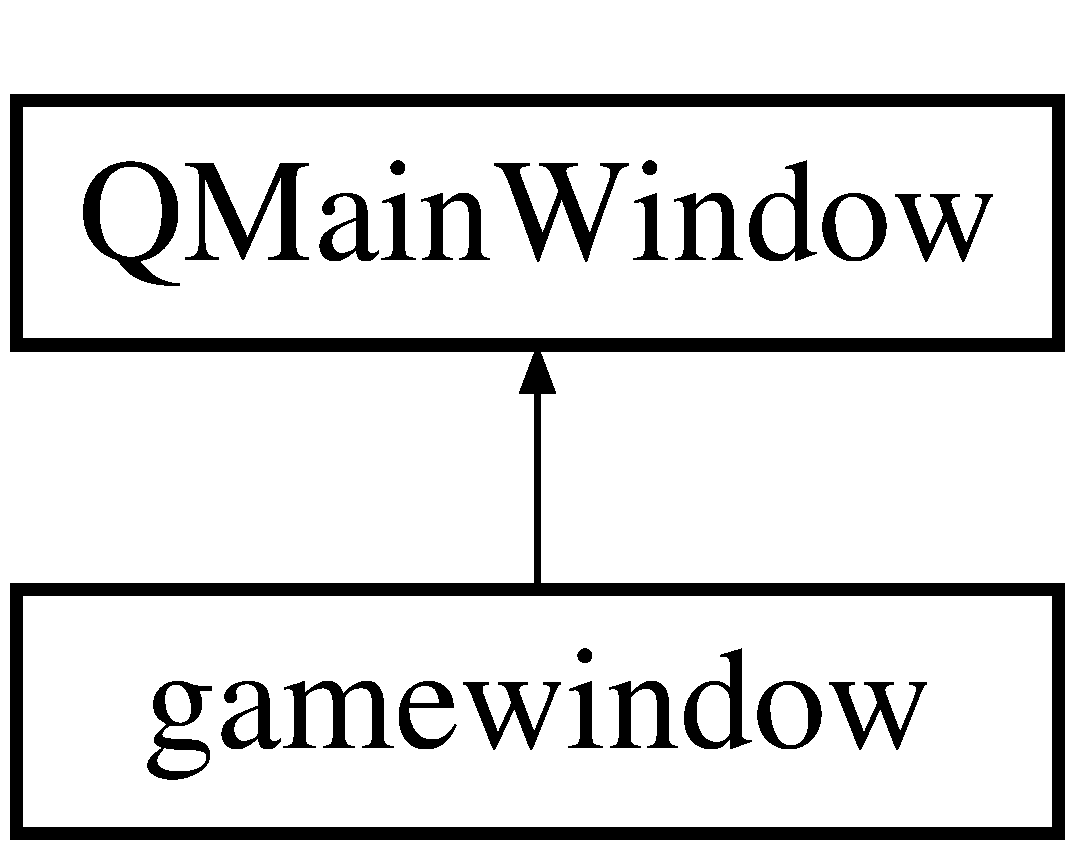
\includegraphics[height=2.000000cm]{classgamewindow}
\end{center}
\end{figure}
\subsection*{Public Slots}
\begin{DoxyCompactItemize}
\item 
\hypertarget{classgamewindow_a69fdf6888c6496deedba54f588867415}{void \hyperlink{classgamewindow_a69fdf6888c6496deedba54f588867415}{move\-Event} ()}\label{classgamewindow_a69fdf6888c6496deedba54f588867415}

\begin{DoxyCompactList}\small\item\em \hyperlink{classgamewindow_a69fdf6888c6496deedba54f588867415}{gamewindow\-::move\-Event} sets up timer function for moving enemies \end{DoxyCompactList}\item 
\hypertarget{classgamewindow_a4a43db9e7606e3e24a63baf6d36a7e79}{void \hyperlink{classgamewindow_a4a43db9e7606e3e24a63baf6d36a7e79}{media\-Event} ()}\label{classgamewindow_a4a43db9e7606e3e24a63baf6d36a7e79}

\begin{DoxyCompactList}\small\item\em \hyperlink{classgamewindow_a69fdf6888c6496deedba54f588867415}{gamewindow\-::move\-Event} sets up timer function for media player for music played in the background \end{DoxyCompactList}\end{DoxyCompactItemize}
\subsection*{Public Member Functions}
\begin{DoxyCompactItemize}
\item 
\hyperlink{classgamewindow_a3e131541b6a8c961d0156a62a02b7862}{gamewindow} (Q\-Widget $\ast$parent=0, bool new\-Game=true, Q\-String session\-Name=N\-U\-L\-L)
\begin{DoxyCompactList}\small\item\em \hyperlink{classgamewindow_a3e131541b6a8c961d0156a62a02b7862}{gamewindow\-::gamewindow} Loads games depending on if its new or saved. Also sets up timer for music to play in the background. The order of the music is randomly picked. \end{DoxyCompactList}\item 
\hypertarget{classgamewindow_ac1f14593e7296da6c62db78f159e48c8}{Q\-Graphics\-View $\ast$ {\bfseries Get\-Graphics\-View} ()}\label{classgamewindow_ac1f14593e7296da6c62db78f159e48c8}

\end{DoxyCompactItemize}
\subsection*{Public Attributes}
\begin{DoxyCompactItemize}
\item 
\hypertarget{classgamewindow_a958cf05885ec517bf2398c9fb2167a20}{int {\bfseries left}}\label{classgamewindow_a958cf05885ec517bf2398c9fb2167a20}

\item 
\hypertarget{classgamewindow_ada0baf8b25d537ad796b6b580201cbf1}{int {\bfseries right}}\label{classgamewindow_ada0baf8b25d537ad796b6b580201cbf1}

\item 
\hypertarget{classgamewindow_aa4b988159a5462c408238bf7ebcc847c}{bool {\bfseries mj\-Has\-Block}}\label{classgamewindow_aa4b988159a5462c408238bf7ebcc847c}

\item 
\hypertarget{classgamewindow_ab95f2fa0cc6ced06d9bb83e6ed1555f5}{Q\-String {\bfseries next\-Level}}\label{classgamewindow_ab95f2fa0cc6ced06d9bb83e6ed1555f5}

\end{DoxyCompactItemize}
\subsection*{Protected Member Functions}
\begin{DoxyCompactItemize}
\item 
\hypertarget{classgamewindow_a403dc8059cacafc856e7a38bb660e161}{void \hyperlink{classgamewindow_a403dc8059cacafc856e7a38bb660e161}{key\-Press\-Event} (Q\-Key\-Event $\ast$event)}\label{classgamewindow_a403dc8059cacafc856e7a38bb660e161}

\begin{DoxyCompactList}\small\item\em \hyperlink{classgamewindow_a403dc8059cacafc856e7a38bb660e161}{gamewindow\-::key\-Press\-Event} listens to keypresses from the user and does an action based on the key that was pressed \end{DoxyCompactList}\end{DoxyCompactItemize}


\subsection{Constructor \& Destructor Documentation}
\hypertarget{classgamewindow_a3e131541b6a8c961d0156a62a02b7862}{\index{gamewindow@{gamewindow}!gamewindow@{gamewindow}}
\index{gamewindow@{gamewindow}!gamewindow@{gamewindow}}
\subsubsection[{gamewindow}]{\setlength{\rightskip}{0pt plus 5cm}gamewindow\-::gamewindow (
\begin{DoxyParamCaption}
\item[{Q\-Widget $\ast$}]{parent = {\ttfamily 0}, }
\item[{bool}]{new\-Game = {\ttfamily true}, }
\item[{Q\-String}]{session\-Name = {\ttfamily NULL}}
\end{DoxyParamCaption}
)\hspace{0.3cm}{\ttfamily [explicit]}}}\label{classgamewindow_a3e131541b6a8c961d0156a62a02b7862}


\hyperlink{classgamewindow_a3e131541b6a8c961d0156a62a02b7862}{gamewindow\-::gamewindow} Loads games depending on if its new or saved. Also sets up timer for music to play in the background. The order of the music is randomly picked. 

gamewindow This class sets up the window for game play. This window loads a new game or a saved game. It also has the keyboard connections set up for the user. 

The documentation for this class was generated from the following files\-:\begin{DoxyCompactItemize}
\item 
gamewindow.\-h\item 
gamewindow.\-cpp\end{DoxyCompactItemize}

\hypertarget{class_graphics_view}{\section{Graphics\-View Class Reference}
\label{class_graphics_view}\index{Graphics\-View@{Graphics\-View}}
}
Inheritance diagram for Graphics\-View\-:\begin{figure}[H]
\begin{center}
\leavevmode
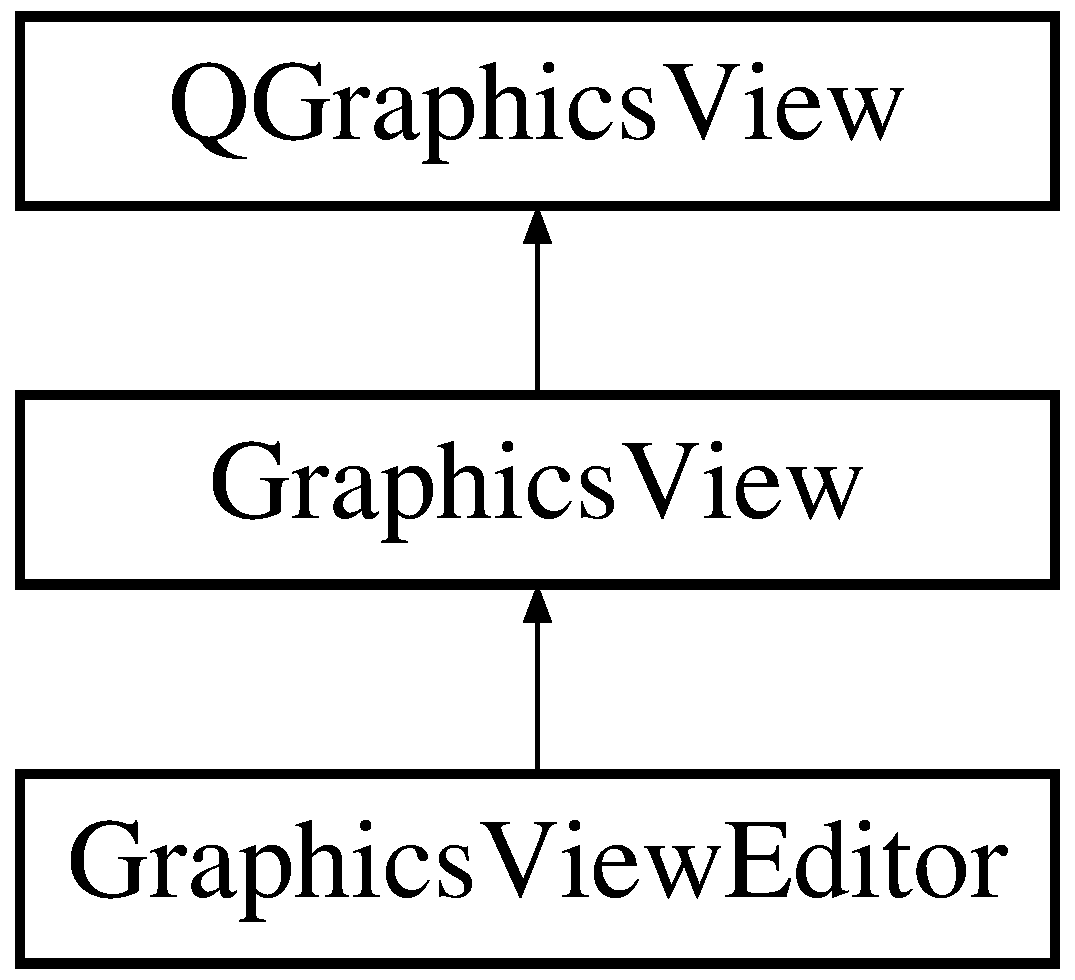
\includegraphics[height=3.000000cm]{class_graphics_view}
\end{center}
\end{figure}


The documentation for this class was generated from the following file\-:\begin{DoxyCompactItemize}
\item 
Doxygen/objects.\-h\end{DoxyCompactItemize}

\hypertarget{class_graphics_view_editor}{\section{Graphics\-View\-Editor Class Reference}
\label{class_graphics_view_editor}\index{Graphics\-View\-Editor@{Graphics\-View\-Editor}}
}
Inheritance diagram for Graphics\-View\-Editor\-:\begin{figure}[H]
\begin{center}
\leavevmode
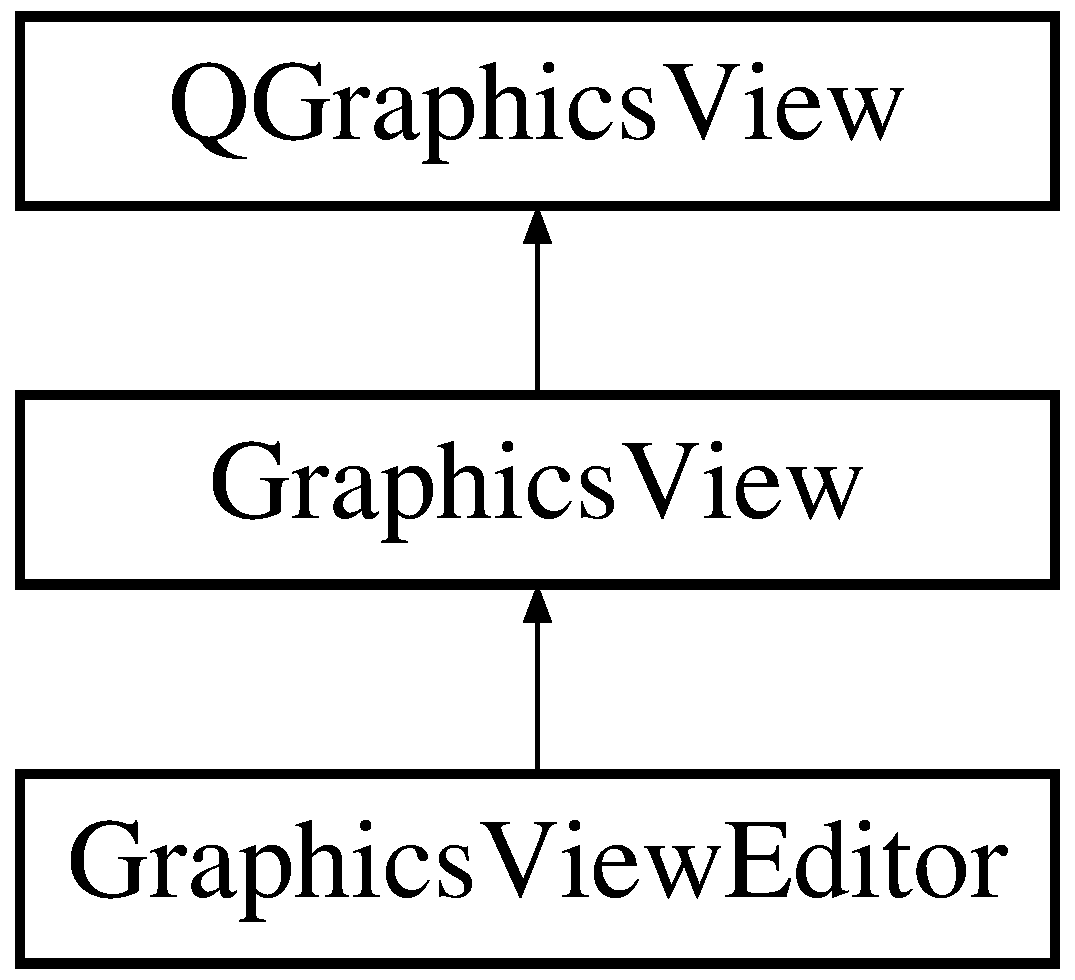
\includegraphics[height=3.000000cm]{class_graphics_view_editor}
\end{center}
\end{figure}
\subsection*{Public Slots}
\begin{DoxyCompactItemize}
\item 
void \hyperlink{class_graphics_view_editor_a6709bc9e3a7f23511cfa0c4db6d92b5a}{mouse\-Press\-Event} (Q\-Mouse\-Event $\ast$event)
\item 
void \hyperlink{class_graphics_view_editor_aeba5b3d56d1e31abe9131476ddd7d20e}{mouse\-Release\-Event} (Q\-Mouse\-Event $\ast$event)
\item 
void \hyperlink{class_graphics_view_editor_a662d6bdadf85a5726a895218d08fdb78}{cell\-Double\-Clicked} (int row, int column)
\end{DoxyCompactItemize}
\subsection*{Public Member Functions}
\begin{DoxyCompactItemize}
\item 
\hyperlink{class_graphics_view_editor_a23421b24ada3080db4b460bf00ac9965}{Graphics\-View\-Editor} (\hyperlink{classengine}{engine} $\ast$gin)
\item 
void \hyperlink{class_graphics_view_editor_a5a50c83ccce7cf211e36507beab4d68a}{Snap\-To\-Grid} ()
\end{DoxyCompactItemize}
\subsection*{Public Attributes}
\begin{DoxyCompactItemize}
\item 
\hypertarget{class_graphics_view_editor_a30d6a7e9b7771e24efbc7e7235b84f08}{bool {\bfseries Auto\-Snap}}\label{class_graphics_view_editor_a30d6a7e9b7771e24efbc7e7235b84f08}

\item 
\hypertarget{class_graphics_view_editor_a9c52faf34ae6a7a894d37de00b1cd73a}{bool {\bfseries m\-Block\-Checked}}\label{class_graphics_view_editor_a9c52faf34ae6a7a894d37de00b1cd73a}

\end{DoxyCompactItemize}
\subsection*{Protected Attributes}
\begin{DoxyCompactItemize}
\item 
\hypertarget{class_graphics_view_editor_ab055e6d90b676077fb391545245aa694}{Q\-Table\-Widget $\ast$ {\bfseries right\-Click\-Menu}}\label{class_graphics_view_editor_ab055e6d90b676077fb391545245aa694}

\end{DoxyCompactItemize}


\subsection{Constructor \& Destructor Documentation}
\hypertarget{class_graphics_view_editor_a23421b24ada3080db4b460bf00ac9965}{\index{Graphics\-View\-Editor@{Graphics\-View\-Editor}!Graphics\-View\-Editor@{Graphics\-View\-Editor}}
\index{Graphics\-View\-Editor@{Graphics\-View\-Editor}!GraphicsViewEditor@{Graphics\-View\-Editor}}
\subsubsection[{Graphics\-View\-Editor}]{\setlength{\rightskip}{0pt plus 5cm}Graphics\-View\-Editor\-::\-Graphics\-View\-Editor (
\begin{DoxyParamCaption}
\item[{{\bf engine} $\ast$}]{gin}
\end{DoxyParamCaption}
)}}\label{class_graphics_view_editor_a23421b24ada3080db4b460bf00ac9965}
\hyperlink{class_graphics_view_editor_a23421b24ada3080db4b460bf00ac9965}{Graphics\-View\-Editor\-::\-Graphics\-View\-Editor} Connects right click to the double right click which is the action desired for adding sprites to the screen. It also connects the picture to the action so that the sprite alone shows on the screen. And it sets up the table for the sprite menu. 

\subsection{Member Function Documentation}
\hypertarget{class_graphics_view_editor_a662d6bdadf85a5726a895218d08fdb78}{\index{Graphics\-View\-Editor@{Graphics\-View\-Editor}!cell\-Double\-Clicked@{cell\-Double\-Clicked}}
\index{cell\-Double\-Clicked@{cell\-Double\-Clicked}!GraphicsViewEditor@{Graphics\-View\-Editor}}
\subsubsection[{cell\-Double\-Clicked}]{\setlength{\rightskip}{0pt plus 5cm}void Graphics\-View\-Editor\-::cell\-Double\-Clicked (
\begin{DoxyParamCaption}
\item[{int}]{row, }
\item[{int}]{column}
\end{DoxyParamCaption}
)\hspace{0.3cm}{\ttfamily [slot]}}}\label{class_graphics_view_editor_a662d6bdadf85a5726a895218d08fdb78}
Graphicsvieweditor The \hyperlink{class_graphics_view_editor}{Graphics\-View\-Editor} is the class that sets up the level editor tool. The class creates a grid menu that displays all of the available sprites for the user tocreate their level. It also defines how the user uses the tool through the mouse.

\hyperlink{class_graphics_view_editor_a662d6bdadf85a5726a895218d08fdb78}{Graphics\-View\-Editor\-::cell\-Double\-Clicked} opens menu of sprites when the leveleditor is right clicked. if a sprite is right clicked the sprite alone is added to the screen. \hypertarget{class_graphics_view_editor_a6709bc9e3a7f23511cfa0c4db6d92b5a}{\index{Graphics\-View\-Editor@{Graphics\-View\-Editor}!mouse\-Press\-Event@{mouse\-Press\-Event}}
\index{mouse\-Press\-Event@{mouse\-Press\-Event}!GraphicsViewEditor@{Graphics\-View\-Editor}}
\subsubsection[{mouse\-Press\-Event}]{\setlength{\rightskip}{0pt plus 5cm}void Graphics\-View\-Editor\-::mouse\-Press\-Event (
\begin{DoxyParamCaption}
\item[{Q\-Mouse\-Event $\ast$}]{event}
\end{DoxyParamCaption}
)\hspace{0.3cm}{\ttfamily [slot]}}}\label{class_graphics_view_editor_a6709bc9e3a7f23511cfa0c4db6d92b5a}
\hyperlink{class_graphics_view_editor_a6709bc9e3a7f23511cfa0c4db6d92b5a}{Graphics\-View\-Editor\-::mouse\-Press\-Event} Connects mouse press signals for clicking the sprite menu and holding the selected sprites \hypertarget{class_graphics_view_editor_aeba5b3d56d1e31abe9131476ddd7d20e}{\index{Graphics\-View\-Editor@{Graphics\-View\-Editor}!mouse\-Release\-Event@{mouse\-Release\-Event}}
\index{mouse\-Release\-Event@{mouse\-Release\-Event}!GraphicsViewEditor@{Graphics\-View\-Editor}}
\subsubsection[{mouse\-Release\-Event}]{\setlength{\rightskip}{0pt plus 5cm}void Graphics\-View\-Editor\-::mouse\-Release\-Event (
\begin{DoxyParamCaption}
\item[{Q\-Mouse\-Event $\ast$}]{event}
\end{DoxyParamCaption}
)\hspace{0.3cm}{\ttfamily [slot]}}}\label{class_graphics_view_editor_aeba5b3d56d1e31abe9131476ddd7d20e}
\hyperlink{class_graphics_view_editor_aeba5b3d56d1e31abe9131476ddd7d20e}{Graphics\-View\-Editor\-::mouse\-Release\-Event()} Allows for dragging the sprite around to position it using the mouse release and it snaps to the grid \hypertarget{class_graphics_view_editor_a5a50c83ccce7cf211e36507beab4d68a}{\index{Graphics\-View\-Editor@{Graphics\-View\-Editor}!Snap\-To\-Grid@{Snap\-To\-Grid}}
\index{Snap\-To\-Grid@{Snap\-To\-Grid}!GraphicsViewEditor@{Graphics\-View\-Editor}}
\subsubsection[{Snap\-To\-Grid}]{\setlength{\rightskip}{0pt plus 5cm}void Graphics\-View\-Editor\-::\-Snap\-To\-Grid (
\begin{DoxyParamCaption}
{}
\end{DoxyParamCaption}
)}}\label{class_graphics_view_editor_a5a50c83ccce7cf211e36507beab4d68a}
\hyperlink{class_graphics_view_editor_a5a50c83ccce7cf211e36507beab4d68a}{Graphics\-View\-Editor\-::\-Snap\-To\-Grid()} Sets up snap to grid so that when sprites are dragged into a position on screen it locks in to the square coordinate position 

The documentation for this class was generated from the following files\-:\begin{DoxyCompactItemize}
\item 
graphicsvieweditor.\-h\item 
graphicsvieweditor.\-cpp\end{DoxyCompactItemize}

\hypertarget{class_main_window}{\section{Main\-Window Class Reference}
\label{class_main_window}\index{Main\-Window@{Main\-Window}}
}
Inheritance diagram for Main\-Window\-:\begin{figure}[H]
\begin{center}
\leavevmode
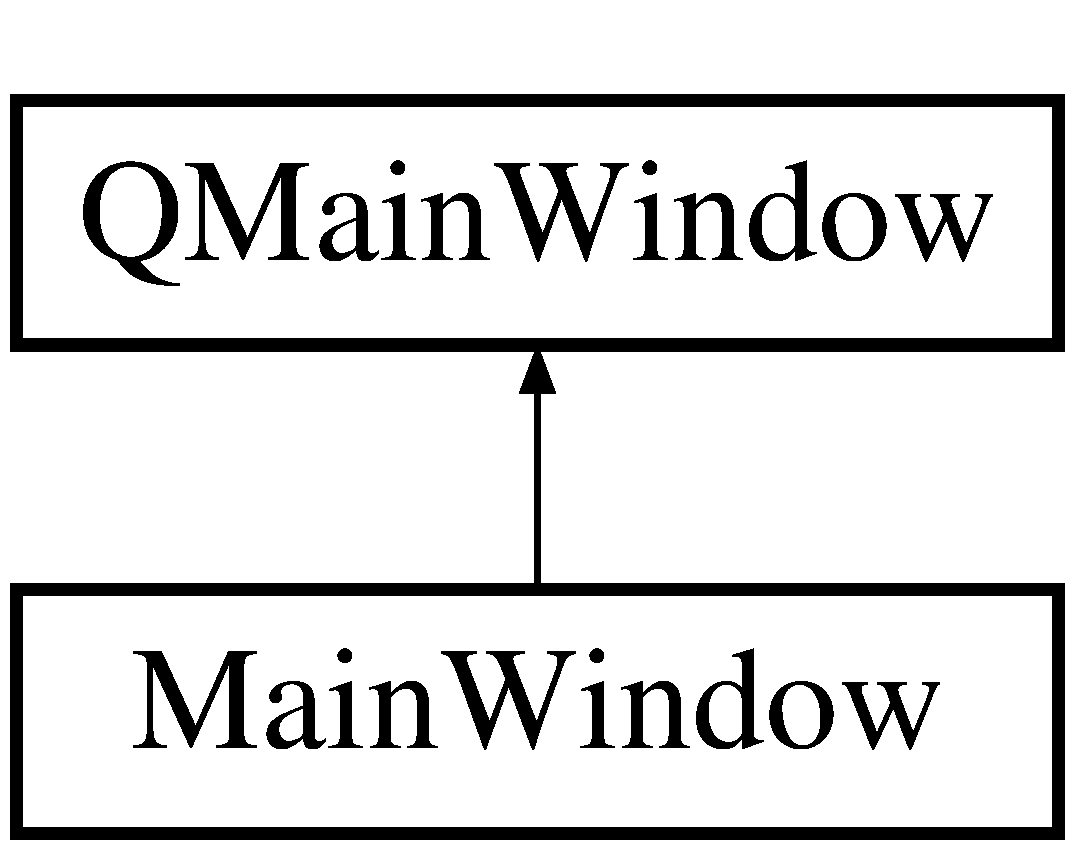
\includegraphics[height=2.000000cm]{class_main_window}
\end{center}
\end{figure}
\subsection*{Public Member Functions}
\begin{DoxyCompactItemize}
\item 
\hypertarget{class_main_window_a100ead45842e8680c9cbfa334a0e30b4}{{\bfseries Main\-Window} (Q\-Widget $\ast$parent=0, \hyperlink{classengine}{engine} $\ast$gin=0, Q\-Graphics\-Scene $\ast$ui\-Scene=N\-U\-L\-L, int B\-L\-O\-C\-K\-\_\-\-S\-I\-Z\-E=30)}\label{class_main_window_a100ead45842e8680c9cbfa334a0e30b4}

\item 
\hypertarget{class_main_window_abbbcd7e315b91ac8ead9d87fa61c9f3c}{void {\bfseries Init\-Graphics} (Q\-Graphics\-Scene $\ast$scene)}\label{class_main_window_abbbcd7e315b91ac8ead9d87fa61c9f3c}

\end{DoxyCompactItemize}


The documentation for this class was generated from the following files\-:\begin{DoxyCompactItemize}
\item 
gamemainwindow.\-h\item 
gamemainwindow.\-cpp\end{DoxyCompactItemize}

\hypertarget{class_my_message_box}{\section{My\-Message\-Box Class Reference}
\label{class_my_message_box}\index{My\-Message\-Box@{My\-Message\-Box}}
}
Inheritance diagram for My\-Message\-Box\-:\begin{figure}[H]
\begin{center}
\leavevmode
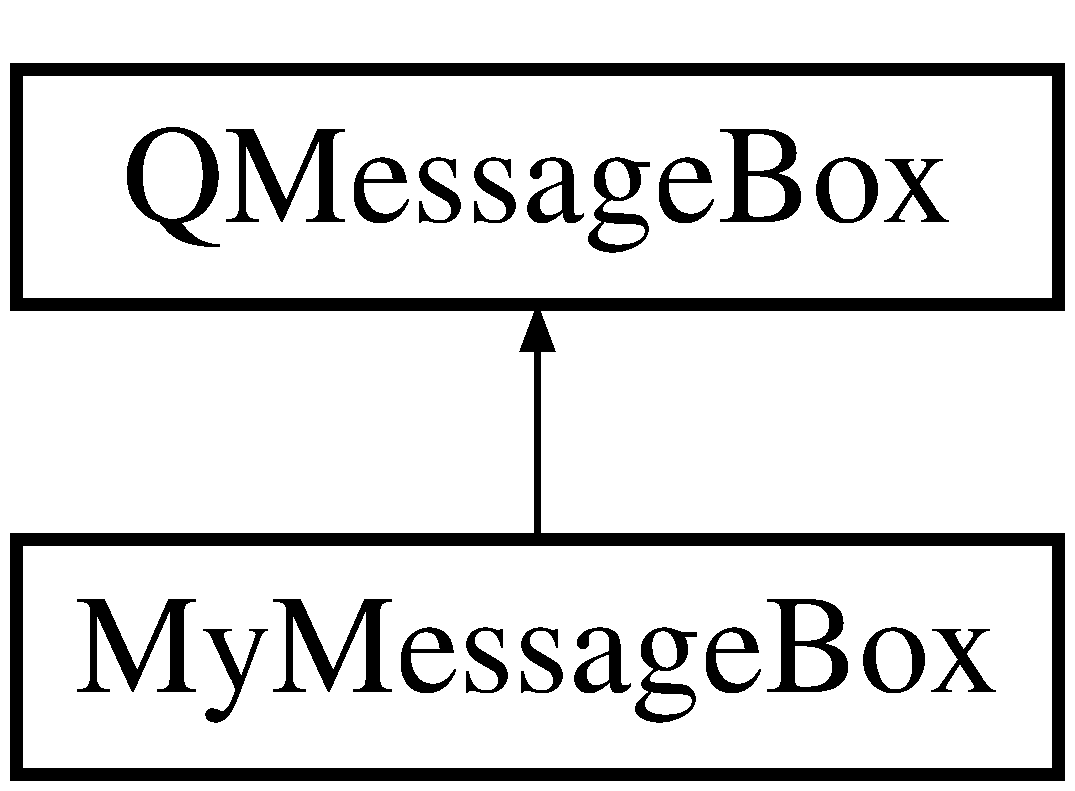
\includegraphics[height=2.000000cm]{class_my_message_box}
\end{center}
\end{figure}
\subsection*{Public Member Functions}
\begin{DoxyCompactItemize}
\item 
\hypertarget{class_my_message_box_a5f2ebba721994e0b991449265daf55fd}{void {\bfseries resize\-Event} ()}\label{class_my_message_box_a5f2ebba721994e0b991449265daf55fd}

\end{DoxyCompactItemize}


The documentation for this class was generated from the following file\-:\begin{DoxyCompactItemize}
\item 
Doxygen/start.\-h\end{DoxyCompactItemize}

\hypertarget{class_node}{\section{Node Class Reference}
\label{class_node}\index{Node@{Node}}
}
\subsection*{Public Member Functions}
\begin{DoxyCompactItemize}
\item 
\hyperlink{class_node_a9187fcac7fd3d010e5a4e66d2ab09ca1}{Node} (Q\-String type, Q\-String location, int x, int y)
\end{DoxyCompactItemize}
\subsection*{Public Attributes}
\begin{DoxyCompactItemize}
\item 
\hypertarget{class_node_a1e3b8be9dd5e9e8ee1515a954eb2a440}{\hyperlink{class_q_graphics_rect_widget}{Q\-Graphics\-Rect\-Widget} $\ast$ {\bfseries sprite}}\label{class_node_a1e3b8be9dd5e9e8ee1515a954eb2a440}

\item 
\hypertarget{class_node_ab67926654974b599162a1d92a8782e77}{Q\-String {\bfseries block\-Type}}\label{class_node_ab67926654974b599162a1d92a8782e77}

\item 
\hypertarget{class_node_a554bf618b49a998f092af1afd298223e}{Q\-String {\bfseries location}}\label{class_node_a554bf618b49a998f092af1afd298223e}

\item 
\hypertarget{class_node_a5e1262ea866e559c23dac491e1a007c4}{Q\-String {\bfseries good\-Obj}}\label{class_node_a5e1262ea866e559c23dac491e1a007c4}

\item 
\hypertarget{class_node_aff1029a518bdc2651007b8856f958364}{int {\bfseries x}}\label{class_node_aff1029a518bdc2651007b8856f958364}

\item 
\hypertarget{class_node_aa3e5b5240023b4528ae85057b3324202}{int {\bfseries y}}\label{class_node_aa3e5b5240023b4528ae85057b3324202}

\item 
\hypertarget{class_node_a6273ae8d26c9b5e8aa400ed25938bd39}{int {\bfseries movement}}\label{class_node_a6273ae8d26c9b5e8aa400ed25938bd39}

\item 
\hypertarget{class_node_af695bd07e0f4b58d85c4ac2fd48cdfa6}{bool {\bfseries has\-Obj}}\label{class_node_af695bd07e0f4b58d85c4ac2fd48cdfa6}

\item 
\hypertarget{class_node_a2559a716f69ccaa76d648d9f1b83065e}{\hyperlink{class_node}{Node} $\ast$ {\bfseries next}}\label{class_node_a2559a716f69ccaa76d648d9f1b83065e}

\item 
\hypertarget{class_node_a632ea91c6a13082308f7692649a68880}{\hyperlink{class_node}{Node} $\ast$ {\bfseries prev}}\label{class_node_a632ea91c6a13082308f7692649a68880}

\end{DoxyCompactItemize}


\subsection{Constructor \& Destructor Documentation}
\hypertarget{class_node_a9187fcac7fd3d010e5a4e66d2ab09ca1}{\index{Node@{Node}!Node@{Node}}
\index{Node@{Node}!Node@{Node}}
\subsubsection[{Node}]{\setlength{\rightskip}{0pt plus 5cm}Node\-::\-Node (
\begin{DoxyParamCaption}
\item[{Q\-String}]{type, }
\item[{Q\-String}]{location, }
\item[{int}]{x, }
\item[{int}]{y}
\end{DoxyParamCaption}
)}}\label{class_node_a9187fcac7fd3d010e5a4e66d2ab09ca1}
obj\-Structue The \hyperlink{classobj_structure}{obj\-Structure} class creates a linked list that contains all of the objects loaded in through the parser. In this case, each objectis a node containing the object type (M\-J, good guy, enemy, block, etc.), position, and picture. 

The documentation for this class was generated from the following files\-:\begin{DoxyCompactItemize}
\item 
Doxygen/obj\-Structure.\-h\item 
Doxygen/obj\-Structure.\-cpp\end{DoxyCompactItemize}

\hypertarget{classobj_structure}{\section{obj\-Structure Class Reference}
\label{classobj_structure}\index{obj\-Structure@{obj\-Structure}}
}
\subsection*{Public Member Functions}
\begin{DoxyCompactItemize}
\item 
\hypertarget{classobj_structure_a471be95d137c9d40b45e49be917f3933}{void {\bfseries add} (Q\-String type, Q\-String location, int x, int y)}\label{classobj_structure_a471be95d137c9d40b45e49be917f3933}

\item 
void \hyperlink{classobj_structure_a4bfcab0d9931a486b303a8be4d7f380a}{add} (Q\-String type, Q\-String location, int x, int y, Q\-String good\-Obj)
\item 
\hypertarget{classobj_structure_ad8ee59f0e4377ee81469edca96b6a623}{void {\bfseries remove} (Q\-String type, int x, int y)}\label{classobj_structure_ad8ee59f0e4377ee81469edca96b6a623}

\item 
void \hyperlink{classobj_structure_a6efb04e79b755dffa27d22a48e51140d}{remove} (\hyperlink{class_node}{Node} $\ast$gone)
\item 
void \hyperlink{classobj_structure_a41750e7cf482a5831d63b4bc0e494101}{remove\-All} ()
\item 
int \hyperlink{classobj_structure_aa7c8aff07ac4acf636029ea3fd9a427b}{get\-Count} ()
\end{DoxyCompactItemize}
\subsection*{Public Attributes}
\begin{DoxyCompactItemize}
\item 
\hypertarget{classobj_structure_aa7c0d7034f8597701ea1317bd6e144b1}{\hyperlink{class_node}{Node} $\ast$ {\bfseries head}}\label{classobj_structure_aa7c0d7034f8597701ea1317bd6e144b1}

\item 
\hypertarget{classobj_structure_ad49ade870fa2a6c48a1f875e9ecbb63b}{\hyperlink{class_node}{Node} $\ast$ {\bfseries tail}}\label{classobj_structure_ad49ade870fa2a6c48a1f875e9ecbb63b}

\end{DoxyCompactItemize}


\subsection{Member Function Documentation}
\hypertarget{classobj_structure_a4bfcab0d9931a486b303a8be4d7f380a}{\index{obj\-Structure@{obj\-Structure}!add@{add}}
\index{add@{add}!objStructure@{obj\-Structure}}
\subsubsection[{add}]{\setlength{\rightskip}{0pt plus 5cm}void obj\-Structure\-::add (
\begin{DoxyParamCaption}
\item[{Q\-String}]{type, }
\item[{Q\-String}]{location, }
\item[{int}]{x, }
\item[{int}]{y, }
\item[{Q\-String}]{good\-Obj}
\end{DoxyParamCaption}
)}}\label{classobj_structure_a4bfcab0d9931a486b303a8be4d7f380a}
obj\-Structure\-::add Adds nodes (objects) to the object list \hypertarget{classobj_structure_aa7c8aff07ac4acf636029ea3fd9a427b}{\index{obj\-Structure@{obj\-Structure}!get\-Count@{get\-Count}}
\index{get\-Count@{get\-Count}!objStructure@{obj\-Structure}}
\subsubsection[{get\-Count}]{\setlength{\rightskip}{0pt plus 5cm}int obj\-Structure\-::get\-Count (
\begin{DoxyParamCaption}
{}
\end{DoxyParamCaption}
)}}\label{classobj_structure_aa7c8aff07ac4acf636029ea3fd9a427b}
\hyperlink{classobj_structure_aa7c8aff07ac4acf636029ea3fd9a427b}{obj\-Structure\-::get\-Count} counts nodes in the object list \hypertarget{classobj_structure_a6efb04e79b755dffa27d22a48e51140d}{\index{obj\-Structure@{obj\-Structure}!remove@{remove}}
\index{remove@{remove}!objStructure@{obj\-Structure}}
\subsubsection[{remove}]{\setlength{\rightskip}{0pt plus 5cm}void obj\-Structure\-::remove (
\begin{DoxyParamCaption}
\item[{{\bf Node} $\ast$}]{gone}
\end{DoxyParamCaption}
)}}\label{classobj_structure_a6efb04e79b755dffa27d22a48e51140d}
obj\-Structure\-::remove removes nodes (objects) from the object list \hypertarget{classobj_structure_a41750e7cf482a5831d63b4bc0e494101}{\index{obj\-Structure@{obj\-Structure}!remove\-All@{remove\-All}}
\index{remove\-All@{remove\-All}!objStructure@{obj\-Structure}}
\subsubsection[{remove\-All}]{\setlength{\rightskip}{0pt plus 5cm}void obj\-Structure\-::remove\-All (
\begin{DoxyParamCaption}
{}
\end{DoxyParamCaption}
)}}\label{classobj_structure_a41750e7cf482a5831d63b4bc0e494101}
\hyperlink{classobj_structure_a41750e7cf482a5831d63b4bc0e494101}{obj\-Structure\-::remove\-All} removes all nodes (objects) from the object list 

The documentation for this class was generated from the following files\-:\begin{DoxyCompactItemize}
\item 
obj\-Structure.\-h\item 
obj\-Structure.\-cpp\end{DoxyCompactItemize}

\hypertarget{classparser}{\section{parser Class Reference}
\label{classparser}\index{parser@{parser}}
}
\subsection*{Public Member Functions}
\begin{DoxyCompactItemize}
\item 
\hyperlink{classparser_ac4cb16e924a735dfb5837772afa1a1a9}{parser} ()
\item 
\hypertarget{classparser_aa16938ad5757d700376a6fadb4e11e2a}{int {\bfseries read\-File} (Q\-Widget $\ast$parent, \hyperlink{classobj_structure}{obj\-Structure} $\ast$good, \hyperlink{classobj_structure}{obj\-Structure} $\ast$enemies, \hyperlink{classobj_structure}{obj\-Structure} $\ast$blocks, \hyperlink{classobj_structure}{obj\-Structure} $\ast$doors, \hyperlink{classobj_structure}{obj\-Structure} $\ast$other, Q\-String file\-Name)}\label{classparser_aa16938ad5757d700376a6fadb4e11e2a}

\item 
\hypertarget{classparser_ace9c694c314e8314bcee42ca751f64a0}{void {\bfseries create\-File} (Q\-String name, \hyperlink{classobj_structure}{obj\-Structure} $\ast$good\-Guys, \hyperlink{classobj_structure}{obj\-Structure} $\ast$enemies, \hyperlink{classobj_structure}{obj\-Structure} $\ast$blocks, \hyperlink{classobj_structure}{obj\-Structure} $\ast$doors, \hyperlink{classobj_structure}{obj\-Structure} $\ast$other)}\label{classparser_ace9c694c314e8314bcee42ca751f64a0}

\end{DoxyCompactItemize}
\subsection*{Public Attributes}
\begin{DoxyCompactItemize}
\item 
\hypertarget{classparser_a60fba17300bd869e168287358a620fc2}{Q\-String {\bfseries cur\-Level}}\label{classparser_a60fba17300bd869e168287358a620fc2}

\item 
\hypertarget{classparser_aded4d171590ab8bc5ff16d28349e72c5}{Q\-String {\bfseries next\-Level}}\label{classparser_aded4d171590ab8bc5ff16d28349e72c5}

\item 
\hypertarget{classparser_a700ed3fe73034eb63ed69dd40f3de7b1}{int {\bfseries lives}}\label{classparser_a700ed3fe73034eb63ed69dd40f3de7b1}

\end{DoxyCompactItemize}


\subsection{Constructor \& Destructor Documentation}
\hypertarget{classparser_ac4cb16e924a735dfb5837772afa1a1a9}{\index{parser@{parser}!parser@{parser}}
\index{parser@{parser}!parser@{parser}}
\subsubsection[{parser}]{\setlength{\rightskip}{0pt plus 5cm}parser\-::parser (
\begin{DoxyParamCaption}
{}
\end{DoxyParamCaption}
)}}\label{classparser_ac4cb16e924a735dfb5837772afa1a1a9}
\hyperlink{classparser_ac4cb16e924a735dfb5837772afa1a1a9}{parser\-::parser} The parser loads the levels as a map for the game. It reads the level file and categorizes each line as a different object (block, door, mj, enemy, etc.). Then it takes in the other information as parameters of the object corresponding to the object picture, location, and type. 

The documentation for this class was generated from the following files\-:\begin{DoxyCompactItemize}
\item 
Doxygen/parser.\-h\item 
Doxygen/parser.\-cpp\end{DoxyCompactItemize}

\hypertarget{class_q_graphics_rect_widget}{\section{Q\-Graphics\-Rect\-Widget Class Reference}
\label{class_q_graphics_rect_widget}\index{Q\-Graphics\-Rect\-Widget@{Q\-Graphics\-Rect\-Widget}}
}
Inheritance diagram for Q\-Graphics\-Rect\-Widget\-:\begin{figure}[H]
\begin{center}
\leavevmode
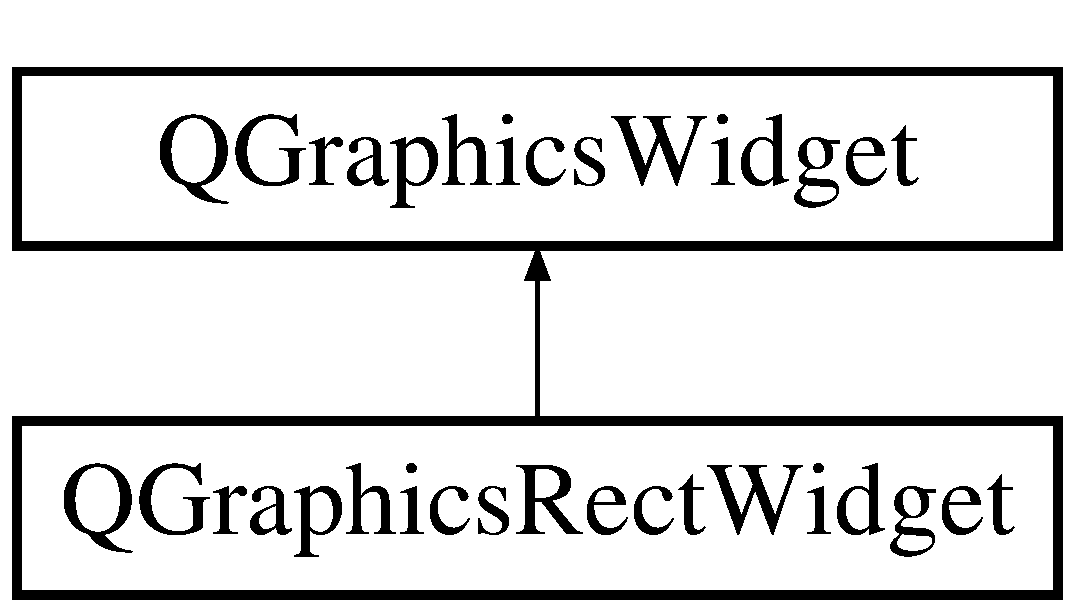
\includegraphics[height=2.000000cm]{class_q_graphics_rect_widget}
\end{center}
\end{figure}
\subsection*{Public Member Functions}
\begin{DoxyCompactItemize}
\item 
\hypertarget{class_q_graphics_rect_widget_a4d6bc01b9a360ff5f8196d1a3469bf0e}{{\bfseries Q\-Graphics\-Rect\-Widget} (Qt\-::\-Global\-Color color, int block\-Width, int block\-Height)}\label{class_q_graphics_rect_widget_a4d6bc01b9a360ff5f8196d1a3469bf0e}

\item 
\hypertarget{class_q_graphics_rect_widget_a6ece45b4d9d1228e752cc33fb114339e}{{\bfseries Q\-Graphics\-Rect\-Widget} (Q\-Pixmap p\-Map, int block\-Width, int block\-Height)}\label{class_q_graphics_rect_widget_a6ece45b4d9d1228e752cc33fb114339e}

\item 
\hypertarget{class_q_graphics_rect_widget_a55d71e9303841da12d016a577efab00f}{{\bfseries Q\-Graphics\-Rect\-Widget} (const char $\ast$sprite\-Name, int block\-Width, int block\-Height)}\label{class_q_graphics_rect_widget_a55d71e9303841da12d016a577efab00f}

\item 
\hypertarget{class_q_graphics_rect_widget_a04a48bc72523408c658e6593ea2b0e0e}{void {\bfseries paint} (Q\-Painter $\ast$painter, const Q\-Style\-Option\-Graphics\-Item $\ast$, Q\-Widget $\ast$)}\label{class_q_graphics_rect_widget_a04a48bc72523408c658e6593ea2b0e0e}

\end{DoxyCompactItemize}
\subsection*{Public Attributes}
\begin{DoxyCompactItemize}
\item 
\hypertarget{class_q_graphics_rect_widget_a72ae5de75dbedb019599f734aa9423c6}{Q\-Brush $\ast$ {\bfseries brush}}\label{class_q_graphics_rect_widget_a72ae5de75dbedb019599f734aa9423c6}

\end{DoxyCompactItemize}


The documentation for this class was generated from the following files\-:\begin{DoxyCompactItemize}
\item 
C\-:/\-Users/\-Joslyn/\-Documents/\-Git\-Hub/\-M\-J\-Baking\-Quest/objects.\-h\item 
C\-:/\-Users/\-Joslyn/\-Documents/\-Git\-Hub/\-M\-J\-Baking\-Quest/objects.\-cpp\end{DoxyCompactItemize}

\hypertarget{classstart}{\section{start Class Reference}
\label{classstart}\index{start@{start}}
}
Inheritance diagram for start\-:\begin{figure}[H]
\begin{center}
\leavevmode
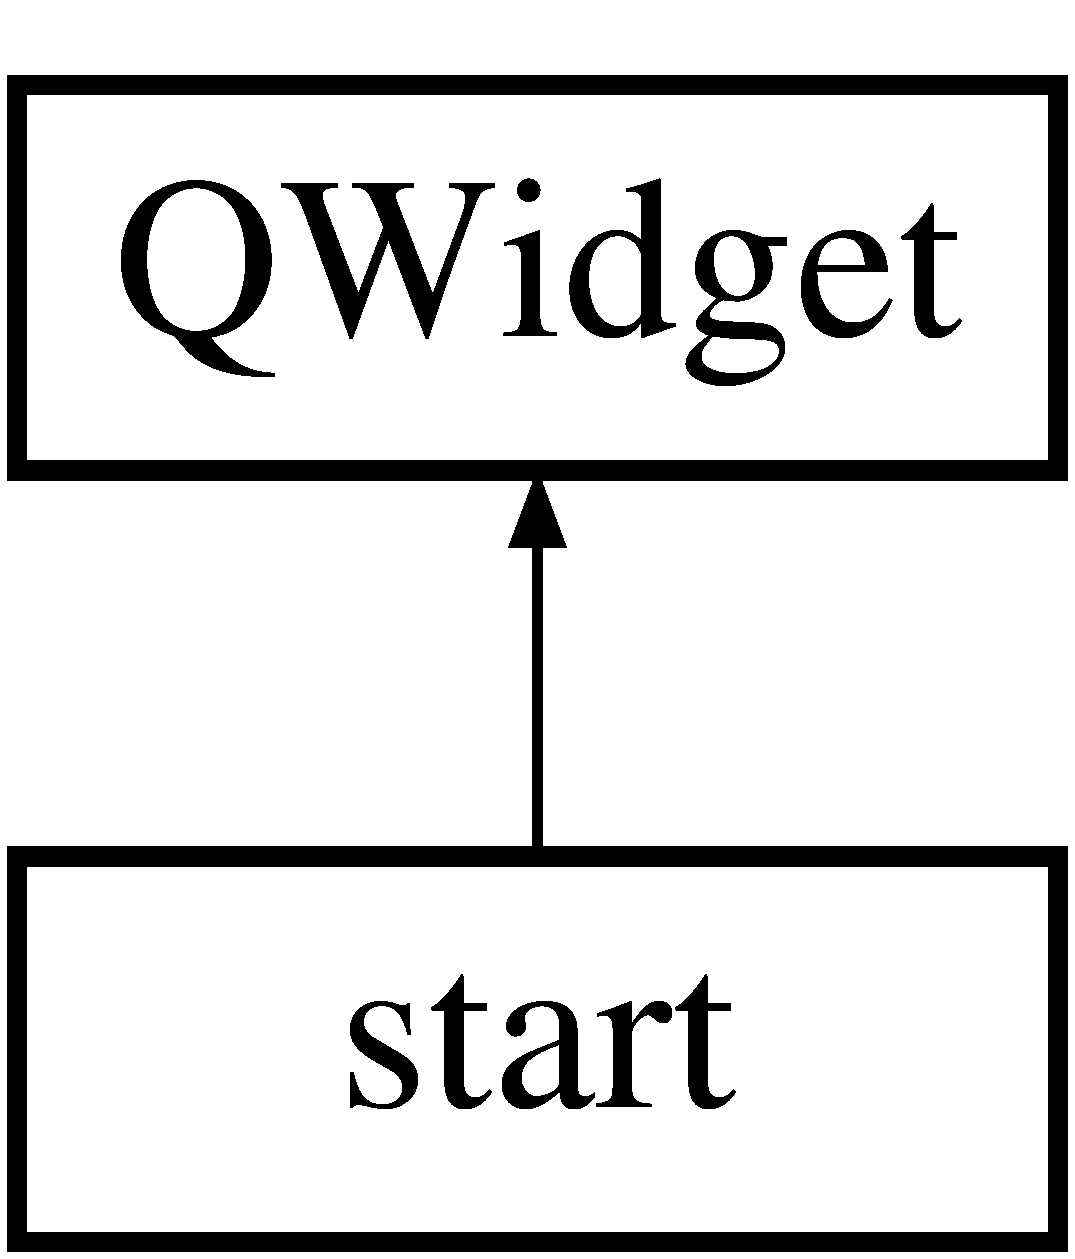
\includegraphics[height=2.000000cm]{classstart}
\end{center}
\end{figure}
\subsection*{Public Member Functions}
\begin{DoxyCompactItemize}
\item 
\hyperlink{classstart_ac258c2204d5abdb20fec5de264236a41}{start} (Q\-Widget $\ast$parent=0)
\end{DoxyCompactItemize}


\subsection{Constructor \& Destructor Documentation}
\hypertarget{classstart_ac258c2204d5abdb20fec5de264236a41}{\index{start@{start}!start@{start}}
\index{start@{start}!start@{start}}
\subsubsection[{start}]{\setlength{\rightskip}{0pt plus 5cm}start\-::start (
\begin{DoxyParamCaption}
\item[{Q\-Widget $\ast$}]{parent = {\ttfamily 0}}
\end{DoxyParamCaption}
)\hspace{0.3cm}{\ttfamily [explicit]}}}\label{classstart_ac258c2204d5abdb20fec5de264236a41}
start This is the start up screen. This class creates a start up window, that links to the game window or the level editor window. The window also includes a help button with instructions for playing the game.

\hyperlink{classstart_ac258c2204d5abdb20fec5de264236a41}{start\-::start} Opens start window and plays start up music 

The documentation for this class was generated from the following files\-:\begin{DoxyCompactItemize}
\item 
start.\-h\item 
start.\-cpp\end{DoxyCompactItemize}

%--- End generated contents ---

% Index
\newpage
\phantomsection
\addcontentsline{toc}{part}{Index}
\printindex

\end{document}
